\documentclass[sigplan,12pt,nonacm=true,review=false]{acmart}
\settopmatter{printfolios=true,printccs=false,printacmref=false}
\usepackage[utf8]{inputenc}
% \usepackage{array}
% \usepackage{booktabs}
\usepackage{tabularx}
\tolerance=1500
\hbadness=1200
\raggedbottom
\title{Analysis of Design Patterns}
\author{HSE Team}{}{}
\email{hsalekh@hse.ru}
\affiliation{%
  \institution{HSE}
  \city{Moscow,Russia}
}
\ccsdesc[300]{Software and its engineering~Software notations and tools~Formal language definitions}
\keywords{OOP, C++, Java, design patterns}
\setlength{\footskip}{14pt}
\setlength{\headheight}{14pt}

\usepackage{graphicx}
\usepackage{amsmath}
\usepackage{attachfile}
\usepackage{wrapfig}

\begin{document}
\begin{abstract}
Design patterns are formalized best practices that the programmer can use to solve common problems when designing an application or system. In this phase of Eolang development, we analyze typical design patterns in Java and C++ by researching multiple popular open-source repositories, to detect common design patterns and their usage statistics and then suggest alternatives in Eolang that could replace such patterns which are not supported in the language. To help us analyse deeper and provide explanation why Eolang alternatives could be better, we implement some of these design patterns in Eolang.
\end{abstract}
\maketitle

\section{Introduction}
This report includes pattern analysis, usage statistics, comparison of design patterns implementation in C++ and Java, implementation of some popular design patterns in Eolang, explanation of why Eolang does not support some design patterns, description of alternatives and explanation of why Eolang alternatives could be better.

\subsection{Backround}
Design is one of the most difficult task in software development \cite{hasheminejad_design_2012} and Developers, who have eagerly adopted them over the past years \cite{wendorff_assessment_2001}, needed to understand not only design patterns \cite{riehle_understanding_1996} but the software systems before they can maintain them, even in cases where documentation and/or design models are missing or of a poor quality. In most cases only the source code as the basic form of documentation is available \cite{streitferdt_searching_2005}. Maintenance is a time-consuming activity within software development, and it requires a good understanding of the system in question. The knowledge about design patterns can help developers to understand the underlying architecture faster. Using design patterns is a widely accepted method to improve software development \cite{hahsler_quantitative_2003}.
A design pattern is a general reusable solution to a commonly occurring \cite{hussain_software_2017} problem in software design \cite{antoniol_object-oriented_2001, coplien_software_1998, noauthor, noauthor_design_nodate-6}. A design pattern isn't a finished design that can be transformed directly into code neither are they static entities, but evolving descriptions of best practices \cite{heer_software_2006}. It is a description or template for how to solve a problem that can be used in many different situations. A design pattern systematically names, motivates, and explains a general design that addresses a recurring design problem in object-oriented systems. It describes the problem, the solution, when to apply the solution, and its consequences. It also gives implementation hints \cite{noauthor_design_2015, schaffer_round-trip_1999}.
Design patterns help to effectively speed up development and engineering processes by providing proven development patterns/paradigms. Quality software design requires considering issues that may not be visible until later in the implementation. Reusing design patterns helps to avoid subtle issues that may be catastrophic and help improve code reliability for programmers and architects familiar with the patterns. 
Design patterns provide general solutions, documented in a format that doesn't require specifics tied to a particular problem. They help software engineers to communicate using well-known, well understood names for software interactions. Common design patterns can be improved over time, making them more robust than ad-hoc designs \cite{noauthor_design_nodate, schmidt_software_1996}. In short, the advantages of design patterns include decoupling a request from specific operations (Chain of Responsibility and Command), making a system independent from software and hardware platforms (Abstract Factory and Bridge), independent from algorithmic solutions (Iterator, Strategy, Visitor), or avoid modifying implementations (Adapter, Decorator, Visitor) \cite{aversano_empirical_2007}. Design patterns, overall, helps to thoroughly and designed well implemented frameworks enabling a degree of software reusability that can significantly improve software quality \cite{pree_design_1997, zhang_what_2012, }.


In this paper, we analyse typical design patterns in Java and C++ and detect common patterns and further look at their usage statistics. There are many design patterns in software development and several of them are common to Java and C++. These design patterns come under three main types.

\section{Design Patterns}
\subsection{Creational design Patterns}
These design patterns are all about class instantiation or object creation. These patterns can be further categorized into Class-creational patterns and object-creational patterns. While class-creation patterns use inheritance effectively in the instantiation process, object-creation patterns use delegation effectively to get the job done. Creational design patterns are the Factory Method, Abstract Factory, Builder, Singleton, Object Pool, and Prototype \cite{kuchana_software_2004, zimmer_relationships_1995}.

\subsubsection{Use case of creational design pattern}
\begin{enumerate}
    \item Suppose a developer wants to create a simple DBConnection class to connect to a database and wants to access the database at multiple locations from code, generally what developer will do is create an instance of DBConnection class and use it for doing database operations wherever required. Which results in creating multiple connections from the database as each instance of DBConnection class will have a separate connection to the database. In order to deal with it, we create DBConnection class as a singleton class, so that only one instance of DBConnection is created and a single connection is established. Because we can manage DB Connection via one instance, we can control load balance, unnecessary connections, etc.
    \item Suppose you want to create multiple instances of similar kind and want to achieve loose coupling then you can go for Factory pattern. A class implementing factory design pattern works as a bridge between multiple classes. Consider an example of using multiple database servers like SQL Server and Oracle. If you are developing an application using SQL Server database as back end, but in future need to change database to oracle, you will need to modify all your code, so as factory design patterns maintain loose coupling and easy implementation, we should go for the factory design pattern in order to achieving loose coupling and the creation of a similar kind of object.
\end{enumerate}

\subsubsection{Factory Method: }
Factory Method, also known as virtual constructor, is a creational design pattern that provides an interface for creating objects in a superclass, but allows subclasses to alter the type of objects that will be created \cite{noauthor_factory_nodate} in a way such that it doesn’t have tight coupling with the class hierarchy of the library \cite{noauthor_design_2015-1}. Factory Method is one of the most used design patterns in Java \cite{noauthor_design_nodate-2}. It is widely used in C++ code and is very useful when you need to provide a high level of flexibility for your code \cite{noauthor_design_nodate-3}.

\subsubsection{Abstract Factory}
Abstract Factory patterns work around a super-factory which creates other factories. Thus, it defines a new Abstract Product Factory for each family of products. This factory is also called as factory of factories. It provides one of the best ways to create an object. Abstract Factory design pattern covers the instantiation of the concrete classes behind two kinds of interfaces, where the first interface is responsible for creating a family of related and dependent products, and the second interface is responsible for creating concrete products. The client is using only the declared interfaces and is not aware which concrete families and products are created \cite{bulajic_approach_2012}. Adding a new family of products affects any existing class that depends on it, and requires complex changes in the existing Abstract Factory code, as well as changes in the application or client code \cite{bulajic_approach_2012}. Bulajic and Jovanovic \cite{bulajic_approach_2012}  demonstrates a solution where adding a new product class does not require complex changes in existing code, and the number of product classes is reduced to one product class per family of related or dependent products.

In Abstract Factory pattern an interface is responsible for creating a factory of related objects without explicitly specifying their classes. Each generated factory can give the objects as per the Factory pattern \cite{noauthor_design_nodate-1}. Abstract Factory pattern is almost similar to Factory Pattern is considered as another layer of abstraction over factory pattern \cite{noauthor_abstract_2017}. 

Abstract factory pattern implementation provides us a framework that allows us to create objects that follow a general pattern. So, at runtime, abstract factory is coupled with any desired concrete factory which can create objects of desired type, \cite{noauthor_abstract_nodate-1}. Fig. \ref{fig:uml1} shows a UML class diagram example for an Abstract Factory Design pattern.

\begin{figure*}[tb]
  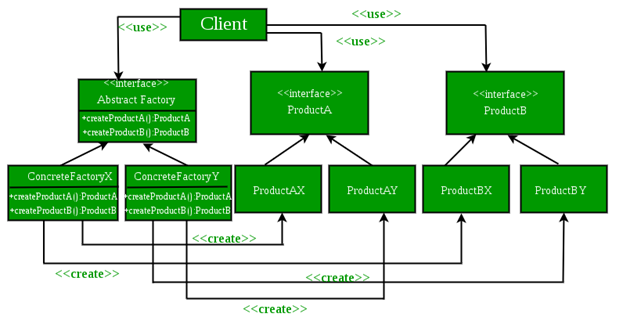
\includegraphics[width=0.8\textwidth]{eolang/tr-02/assets/Picture1.png}
  \caption{UML class diagram example for the Abstract Factory Design Pattern}
  \label{fig:uml1}
\end{figure*}

This pattern is particularly useful when the client doesn’t know exactly what type to create. The Abstract Factory pattern helps you control the classes of objects that an application creates by isolating concrete classes. The class of a concrete factory appears only once in an application, that is where it’s instantiated. This makes it easy to change the concrete factory an application uses. Abstract Factory makes this easy for an application use object from only one family at a time when product objects in a family are designed to work together. 
Abstract Factory interface fixes the set of products that can be created. This serves as a disadvantage because extending abstract factories to produce new kinds of Products is not easy. 
The abstract factory design pattern can be implemented in both Java and C++ as demonstrated at \cite{noauthor_abstract_2017, noauthor_abstract_nodate}. The Abstract Factory pattern is pretty common in C++ code. Many frameworks and libraries use it to provide a way to extend and customize their standard components



\subsubsection{Builder}
Builder pattern builds a complex object using simple objects and using a step-by-step approach and the final step will return the object. The builder is independent of other objects. Fig. 2 show a UML diagram of builder design pattern. Immutable objects can be build without much complex logic in object building process. Builder design pattern also helps in minimizing the number of parameters in constructor and thus there is no need to pass in null for optional parameters to the constructor. As a disadvantage, it requires creating a separate ConcreteBuilder for each different type of Product \cite{noauthor_design_nodate-4, noauthor_builder_2017}.

\subsubsection{Singleton}
In software engineering, the term singleton implies a class which can only be instantiated once, and a global point of access to that instance is provided \cite{noauthor_abstract_nodate-1}. This pattern involves a single class which is responsible to create an object while making sure that only single object gets created. It one of the simplest design patterns in Java and C++.

\subsubsection{Object Pool}
Object pool pattern is a software creational design pattern which is used in situations where the cost of initializing a class instance is very high. An Object pool is a container which contains some number of objects. So, when an object is taken from the pool, it is not available in the pool until it is put back.

\subsubsection{Prototype}
Prototype pattern refers to creating duplicate object while keeping performance in mind. This pattern involves implementing a prototype interface which tells to create a clone of the current object.

\subsection{Structural}
These design patterns are about organizing different classes and objects to form larger structures and provide new functionality. Structural design patterns are Adapter, Bridge, Composite, Decorator, Facade, Flyweight, Private Class Data, and Proxy \cite{kuchana_software_2004, zimmer_relationships_1995}.

\subsubsection{Use Case of Structural Design Pattern}
When 2 interfaces are not compatible with each other and want to establish a relationship between them through an adapter it’s called an adapter design pattern. Adapter pattern converts the interface of a class into another interface or class that the client expects, i.e adapter lets classes works together that could not otherwise because of incompatibility. So, in these types of incompatible scenarios, we can go for the adapter pattern.

\subsubsection{Adapter}
Adapter design pattern allows objects with incompatible interfaces to collaborate \cite{tichy_catalogue_1997}. Adapter pattern works as a bridge between those two incompatible interfaces. A real-life example could be a case of card reader which acts as an adapter between memory card and a laptop. You plugin the memory card into card reader and card reader into the laptop so that memory card can be read via laptop \cite{noauthor_design_nodate-5}.  

\subsubsection{Bridge}
The bridge pattern is used when we need to decouple \cite{wendorff_assessment_2001} an abstraction from its implementation so that the two can vary independently \cite{tichy_catalogue_1997}. It helps you split a large class or a set of closely related classes into two separate hierarchies—abstraction and implementation—which can be developed independently of each other. 

\subsubsection{Composite}
Composite design pattern helps in composing objects into tree structures and then work with these structures as if they were individual objects. It is used where a group of objects need to be treated in similar way as a single object. This pattern creates a class that contains group of its own objects and provides ways to modify this group of same objects. 

\subsection{Decorator}
Decorator design pattern allows a user to add new functionality to an existing object without altering its structure. It allows the attachment of new behaviours to objects by placing these objects inside special wrapper objects that contain the behaviours. 

\subsubsection{Facade}
Facade design pattern, as the name goes, hides the complexities of the system and provides an interface to the client by which the client can access the system. It provides a simplified interface to a library, a framework, or any other complex set of classes. In essence, it provides methods required by the client and delegates calls to methods of existing system classes. 

\subsubsection{Flyweight}
The Flyweight pattern enables you to fit more objects into the available amount of RAM by sharing common parts of state between multiple objects instead of keeping all the data in each object. It is primarily used to reduce the number of objects created and to decrease memory footprint and increase performance.

\subsubsection{Private Class Data}
Private Class Data is used to encapsulate class data and control write access to class attributes as it separates data from methods that us it. 

\subsubsection{Proxy}
The Proxy pattern controls access to the original object \cite{wendorff_assessment_2001}, allowing you to perform something either before or after the request gets through to the original object. It represents functionality of another class.

\subsection{Behavioural}
Behavioral patterns are about identifying common communication patterns between objects and realizing these patterns. Behavioral patterns are Chain of responsibility, Command, Interpreter, Iterator, Mediator, Memento, Null Object, Observer, State, Strategy, Template method and Visitor \cite{kuchana_software_2004, zimmer_relationships_1995}.

\subsubsection{Use Case of Behavioral Design Pattern}
The template pattern defines the skeleton of an algorithm in an operation deferring some steps to sub-classes. The template method lets subclasses redefine certain steps of an algorithm without changing the algorithm structure. For example, in your project, you want the behavior of the module to be able to extend, such that we can make the module behave in new and different ways as the requirements of the application change, or to meet the needs of new applications. However, no one is allowed to make source code changes to it, i.e. you can add but can’t modify the structure in those scenarios a developer can approach template design pattern \cite{noauthor_design_nodate, noauthor_design_2015}.

Sample implementation of these patterns \cite{noauthor_huston_nodate} are available here in both Java and C++.

\subsubsection{Chain of responsibility}
Chain of responsibility pattern suggests a chain of receiver objects for a request. It decouples sender and receiver of a request based on type of request. It allows you to pass requests along a chain of handlers. Upon receiving a request, each handler decides either to process the request or to pass it to the next handler in the chain.

\subsubsection{Command}
Command pattern is also known as action or transaction pattern. This pattern turns a request into a stand-alone object that contains all information about the request. The transformation allows you pass requests as a method argument, delay or queue a request’s execution, and support undoable operations. It is data driven and it wraps an object under an object as command \cite{wendorff_assessment_2001} and passes it to invoker object. Invoker object looks for the appropriate object which can handle this command and passes the command to the corresponding object which executes the command.

\subsubsection{Interpreter}
Interpreter pattern provides a way to evaluate language grammar or expression. Given a language, interpreter defines a representation for the language’s grammar along with an interpreter that uses the representation to interpret sentences in the language. Then it maps a domain to a language, the language to a grammar, and the grammar to a hierarchical object-oriented design. This pattern is used in SQL parsing, symbol processing engine etc. 
The Iterator pattern is very commonly used design pattern in Java and .Net programming environment. It allows sequential traversal through a complex data structure without exposing its internal details \cite{tichy_catalogue_1997}. This pattern is also common in C++ code. Mediator is used to reduce communication complexity between multiple objects or classes by providing a mediator class which normally handles all the communications between different classes and supports easy maintenance of the code by loose coupling \cite{tichy_catalogue_1997}. It encapsulates how a set of objects interact.

\subsubsection{Memento}
Memento pattern is used to restore state of an object to a previous state. Without violating encapsulation, you can capture and externalize an object's internal state so that the object can be returned to this state later. 

\subsubsection{Null Object}
In Null Object pattern, a null object replaces check of NULL object instance. The intent of a Null Object is to encapsulate the absence of an object by providing a substitutable alternative that offers suitable default do-nothing behaviour in case data is not available.

\subsubsection{Observer}
Observer pattern is used when there is one-to-many relationship between objects such as if one object is modified, its dependent objects are to be notified automatically \cite{wendorff_assessment_2001}. 

\subsubsection{State}
In State pattern, objects are created to represent various states and a context object whose behaviour varies as its state object changes. So, in State pattern, a class behaviour changes based on changes in its internal state. 

\subsubsection{Strategy}
Strategy design pattern is the pattern where a class behaviour or its algorithm can be changed at run time. 

\subsubsection{Template}
In Template pattern, an abstract class exposes defined way(s)/template(s) to execute its methods. Its subclasses can override the method implementation as per need, but the invocation is to be in the same way as defined by an abstract class. It allows the algorithm to vary independently from the clients that use it. 

\subsubsection{Visitor}
In Visitor pattern, a visitor class changes the executing algorithm of an element class. By this way, execution algorithm of element can vary as and when visitor varies. Visitor allows the definition of a new operation without changing the classes of the elements on which it operates.


\section{Criticism}
The concept of design patterns has been criticized by some in the field of computer science.

\subsection{Targets the wrong problem}
The need for patterns results from using computer languages or techniques with insufficient abstraction ability. Under ideal factoring, a concept should not be copied, but merely referenced. But if something is referenced instead of copied, then there is no "pattern" to label and catalog. Paul Graham writes in the essay Revenge of the Nerds \cite{noauthor_design_nodate}.

Peter Norvig provides a similar argument. He demonstrates that 16 out of the 23 patterns in the Design Patterns book (which is primarily focused on C++) are simplified or eliminated (via direct language support) in Lisp or Dylan.

\subsection{Lacks formal foundations}
The study of design patterns has been excessively ad hoc, and some have argued that the concept sorely needs to be put on a more formal footing. At OOPSLA 1999, the Gang of Four were (with their full cooperation) subjected to a show trial, in which they were "charged" with numerous crimes against computer science. They were "convicted" by $\frac{2}{3}$ of the "jurors" who attended the trial.

\subsection{Leads to inefficient solutions}
The idea of a design pattern is an attempt to standardize what are already accepted best practices. In principle this might appear to be beneficial, but in practice it often results in the unnecessary duplication of code. It is almost always a more efficient solution to use a well-factored implementation rather than a "just barely good enough" design pattern \cite{noauthor_design_nodate}.

\subsection{Does not differ significantly from other abstractions}
Some authors allege that design patterns don't differ significantly from other forms of abstraction, and that the use of new terminology (borrowed from the architecture community) to describe existing phenomena in the field of programming is unnecessary. The Model-View-Controller paradigm is touted as an example of a "pattern" which predates the concept of "design patterns" by several years. It is further argued by some that the primary contribution of the Design Patterns community (and the Gang of Four book) was the use of Alexander's pattern language as a form of documentation; a practice which is often ignored in the literature \cite{noauthor_design_nodate}.

According to [36], generality, precision, and understandability are the most important goals to consider in order to simplify software design pattern description.

\section{Common design patterns in popular open-source repositories and their usage statistics}
Hahsler \cite{hahsler_quantitative_2003} analyses the application of design patterns in Java by identifying patterns in projects using their log messages to look for names and descriptions. This attempt was done based on the idea that the names of design patterns become part of a common design language which developers  use  to  communicate more  efficiently. Fig. \ref{fig:stats1} shows the graph of the usage statistics according the approach of Hahsler \cite{hahsler_quantitative_2003}.

\begin{figure*}[!t]
  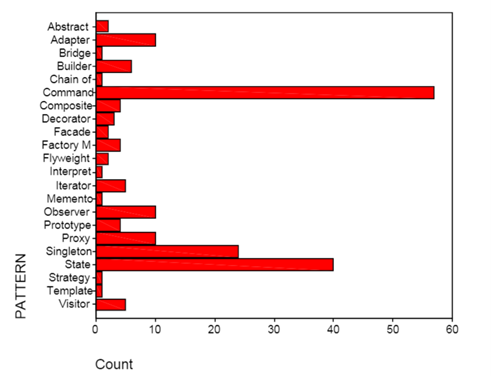
\includegraphics[width=0.8\textwidth]{eolang/tr-02/assets/Picture3.png}
  \caption{Number of Java Projects using individual design patterns \cite{hahsler_quantitative_2003}}
  \label{fig:stats1}
\end{figure*}


Vokac \cite{vokac_defect_2004} analysed the weekly evolution and maintenance of a large commercial product (C++, 500,000 LOC) over three years, comparing defect rates for classes that participated in selected design patterns to the code at large. He extracted design pattern information and concluded that Observer and Singleton patterns are correlated with larger code structures. The Template Method pattern was used in both simple and complex situations, leading to no clear tendency. The frequencies of pattern occurrence are shown in table \ref{tab:stats2}.
\footnotesize
\begin{table}[]
    \centering
    \begin{tabularx}{\linewidth}{p{0.57\linewidth}|r|r|}
         Patterns&Occurrences&\%  \\ \hline
         No Pattern&183634&77.5\% \\ \hline
         Factory&20237&8.5\% \\
         Singleton&3331&1.4\% \\
         Observer&16061&6.8\% \\ 
         Template Method&5381&2.3\% \\
         Decorator&1513&0.6\% \\ \hline
         
         Factory + Observer + Singleton&485&0.2\% \\
         Observer + Template&953&0.4 \% \\
         Observer + Singleton&2390&1.0\% \\
         Factory + Observer&612&0.3\% \\
         Factory + Singleton&2279&1.0% \\ \hline
         
    \end{tabularx}
    \caption{Frequencies of Pattern Occurrences and Percentage of Code Covered by the Patterns}
    \label{tab:stats2}
\end{table}

\section{Comparison of Design Patterns in C++ and Java}
See Table \ref{tab:comparison}.
\footnotesize
\begin{table*}[htbp]
    \centering
    \begin{tabularx}{\textwidth}{|l|p{0.12\linewidth}|p{0.35\linewidth}|p{0.35\linewidth}|}
    \hline
    Category & Pattern & Java & C++ \\ \hline
    Creational & Factory method & Uses abstract keyword to declare factory methods in factory classes to be later implemented by subclasses & Uses static pointers to declare factory methods \\ \hline
    
    &Abstract factory&Uses ‘abstract’ keyword to make abstract factories classes and interfaces&Uses ‘class’ keyword and pointers to create abstract factories and the ‘new’ keyword to create concrete factories which is later used to create concrete objects  \\ \hline
    
    &Builder&Defines classes with creation methods for creating or building complex objects.&An abstract base class declares the standard construction process, and concrete derived classes define the appropriate implementation for each step of the process. Uses struct and class keyword in process. \\ \hline
    
    &Singleton&Uses the public keyword to define a single point of access method for classes&Make the class responsible for its own global pointer and "initialization on first use" (by using a private static pointer and a public static accessor method) \\ \hline
    
    &Prototype &Uses the cloneable interface for implementing class prototypes&A superclass defines a clone method and subclasses implement this method to return an instance of the class \\ \hline
    
    
    Structural&Adapter&The adapter class uses the extend keyword to extend another class to make it compatible with another class&An abstract base class is created that specifies the desired interface. An "adapter" class is defined that publicly inherits the interface of the abstract class, and privately inherits the implementation of the legacy component. This adapter class "maps" or "impedance matches" the new interface to the old implementation. \\ \hline
    
    &Bridge&Use abstraction and implementation to decouple classes into several related hierarchies&Uses abstraction and implementation \\ \hline
    
    &Composite&Uses inheritance to hierarchically implement an object tree&Uses inheritance and polymorphism to implement scalar/primitive classes and vector/container classes  \\ \hline
    
    &Decorator&Uses interface keyword to wrap subclasses and allow the subclasses to dynamically add new behaviours to objects&Uses the concept of wrapping-delegation which involves pointers to help add new behaviours to objects dynamically \\ \hline
    
    
    Behavioural&Chain of responsibility&Defines an abstract class with series of methods including abstract methods for other classes to implement and handle a chain of actions independently&Uses pointers and classes and defines a chain method in the base class for delegating to the next object. \\ \hline
    
    &Command&Applies the concept of inheritance and encapsulation to turn actions into objects&Applies the concept of inheritance and encapsulation to turn actions into objects \\ \hline
    &Observer&Defines event listeners based on inheritance and encapsulation&Models the "independent" functionality with a "subject" abstraction and Models the "dependent" functionality with "observer" hierarchy \\ \hline
    
    &Null object&Encapsulates the absence of an object by providing a substitutable alternative that offers suitable default do nothing behaviour&Similarly, provides a class that checks for null and returns a boolean \\ \hline
    
    &Mediator&Uses ‘interface’ keyword to declare mediators which are later implemented by classes that intend to communicate with each other&Uses classes and pointers to implement mediators \\ \hline

    \end{tabularx}
    \caption{Comparison of Design Patterns in C++ and Java}
    \label{tab:comparison}
\end{table*}

\section{Implementation of Some Design Patterns in Eolang}
\subsection{Abstract Factory}
An abstract factory is a pattern that generates objects.

\subsubsection{Purpose}
Provides an interface for creating families of interconnected or interdependent objects without specifying their specific classes.

\subsubsection{Structure}
See Fig \ref{fig:5}.
\begin{figure*}[!t]
  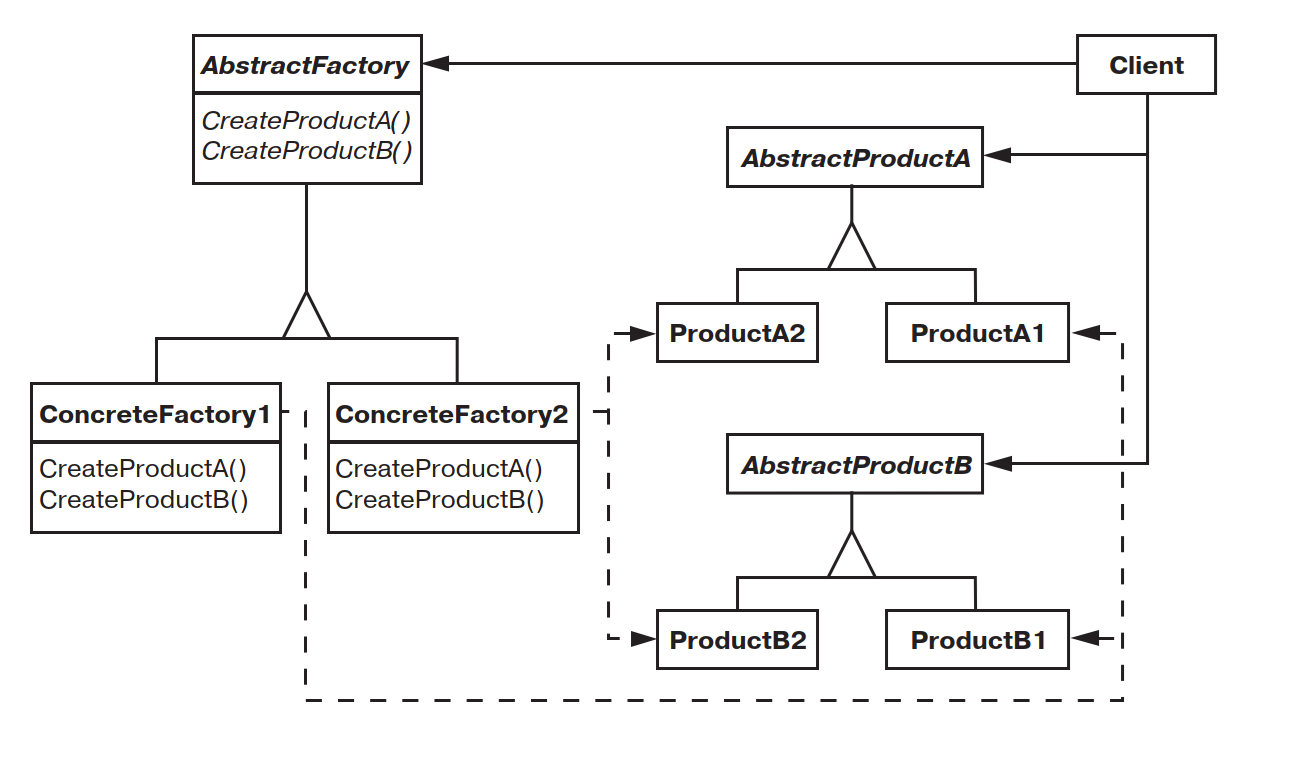
\includegraphics[width=0.8\textwidth]{eolang/tr-02/assets/Picture5.png}
  \caption{Abstract Factory}
  \label{fig:5}
\end{figure*}

\subsubsection{Participants}
\begin{enumerate}
    \item AbstractFactory — abstract factory: declares an interface for operations that create abstract product objects.
    \item ConcreteFactory — specific factory: implements operations that create specific objects-products.
    \item AbstractProduct — abstract product: declares the interface for the type of object-product.
    \item ConcreteProduct — specific product: defines the product object created by the corresponding particular factory, and implements the AbstractProductinterface.
    \item Client: uses only interfaces that are declared in the AbstractFactory and  AbstractProductclasses.
\end{enumerate}

\subsubsection{Implementation}
\begin{verbatim}
1.	+package sandbox
2.	+alias stdout org. eolang. io. stdout
3.	+alias sprintf org.eolang.txt.sprintf
4.	
5.	[type] > abstractFactory
6.	  if. > concreteFactory
7.	    eq.
8.	      type
9.	      "1"
10.	    concreteFactory1
11.	    concreteFactory2
12.	
13.	  [] > createProductA
14.	    createProductA. > @
15.	      ^.concreteFactory
16.	  [] > createProductB
17.	    createProductB. > @
18.	      ^.concreteFactory
19.	
20.	[] > concreteFactory1
21.	  [] > createProductA
22.	    1 > @
23.	  [] > createProductB
24.	    2 > @
25.	
26.	[] > concreteFactory2
27.	  [] > createProductA
28.	    "one" > @
29.	  [] > createProductB
30.	    "two" > @
31.	
32.	[args...] > appAbstractFactory
33.	  abstractFactory > objFactory
34.	    args.get 0
35.	  stdout > @
36.	    sprintf
37.	      "ProductA: %s\nProductB: %s\n"
38.	      objFactory.createProductA
39.	      objFactory.createProductB 

\end{verbatim}


\textbf{Output}
\begin{verbatim}
$ ./run.sh 1
ProductA: 1
ProductB: 2
$ ./run.sh 2
ProductA: one
ProductB: two
\end{verbatim}


This program creates objects of integers or strings depending on the args parameter [0]. If  args[0] = 1, then objects 1 and 2 will be created, otherwise -  "one"  and  "two".
The template assumes the use of interfaces that are not present in the  EO. In this case, an attempt was made to implement the interface through the EO  object has a type parameter depending on which a specific implementation of the object factory is selected. This makes the interface object dependent on the set of implementations of this interface (when adding anew implementation, you must make changes to the interface object).

\subsection{Singleton (singles)}
A singleton is a pattern that generates objects.

\subsubsection{Purpose}
Ensures that the class has only one instance and provides a global access point to it.

\subsubsection{Structure}
See fig. \ref{fig:singleton}.
\begin{figure}
    \centering
    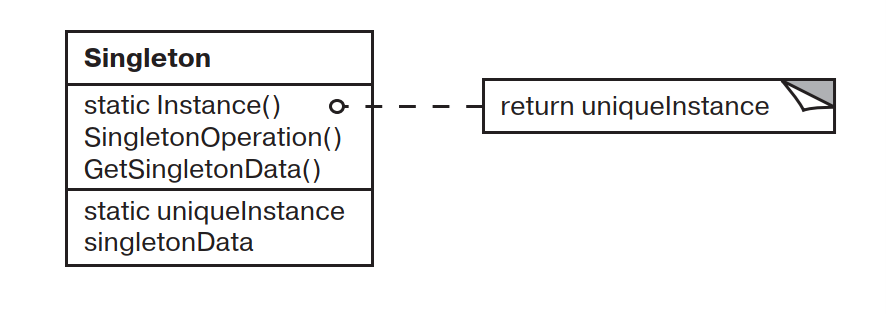
\includegraphics{eolang/tr-02/assets/Picture6.png}
    \caption{Singleton Design Pattern}
    \label{fig:singleton}
\end{figure}

\subsubsection{Participants}
Singleton Singleton:
\begin{enumerate}
    \item Defines an Instance operation that allows clients to access a single instance. Instance is a class operation,  that is,  a static method of a class
    \item May be responsible for creating your own unique instance.
\end{enumerate}

\subsubsection{Relations}
Clients access an instance of the Singleton class only through its Instance operation. 

\subsubsection{Implementation}
There are no classes in the EO, so this pattern is not implemented in its pure form. If we define Singleton in  terms  of  EO as an object that is guaranteed to have only one copy, then the implementation of this object is also impossible for the following reasons:
\begin{enumerate}
    \item There are no references in the EO.  Any use of an object in a location other than the place of definition is a copy of this object.
    \item EO  does not have the ability to restrict access to objects or prevent it from being copied. You cannot restrict the creation of copies of an object.

\end{enumerate}

\subsection{Prototype}
A prototype is a pattern that generates objects.

\subsubsection{Purpose}
Specifies the types of objects to create using the prototype instance and creates new objects by copying the prototype.

\subsubsection{Structure}
See fig \ref{fig:7}.
\begin{figure*}
    \centering
    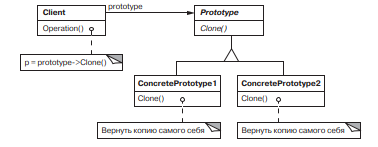
\includegraphics[width=0.8\textwidth]{eolang/tr-02/assets/Picture7.png}
    \caption{Prototype Design Pattern}
    \label{fig:7}
\end{figure*}

\begin{enumerate}
    \item — prototype: declares an interface for cloning itself.
    \item — Concrete Prototype: implements the operation of cloning itself.
    \item  — client: creates a new object by asking the prototype to clone itself.
\end{enumerate}

\subsubsection{Implementation}
In Eolang, each object can be copied, and each object can perform template functions.

\subsection{Observer}
In EO, all objects have immutable state. Based on the purpose of the template, its use in EO is pointless.

\subsection{Bridge}
A bridge is a pattern that structures objects.

\subsubsection{Purpose}
Separate abstraction from its implementation so that both can be changed independently.

\subsubsection{Structure}
See fig. \ref{fig:8}
\begin{figure*}
    \centering
    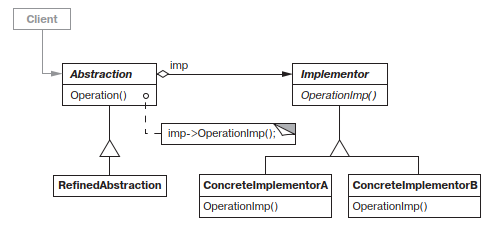
\includegraphics[width=0.8\textwidth]{eolang/tr-02/assets/Picture8.png}
    \caption{Bridge Design Pattern}
    \label{fig:8}
\end{figure*}

\subsubsection{Participants}
\begin{enumerate}
    \item Abstraction — abstraction: defines the abstraction interface, and stores a reference to an object of type Implementor.
    \item RefinedAbstraction —  refined abstraction: extends the interface defined by abstraction abstraction.
    \item Implementor — implementer: defines the interface for the implementation classes. it does not have to exactly match the interface of the abstraction class. In fact both interfaces can be completely different. usually the interface of the Implementor class provides only primitive operations, and the  Abstraction class defines higher-level operations based on these primitives.
    \item ConcreteImplementor —  specific implementer: implements the interface of the Implementor class and defines its specific implementation.
\end{enumerate}

\subsubsection{Relations}
The Abstraction object redirects client requests to its  Implementor object.

\subsection{Chain of responsibility}
A chain of responsibilities is a pattern of behavior of objects.

\subsubsection{Purpose}
Avoids binding the sender of the request to its recipient by providing the ability to process the request to multiple objects. Binds the receiving objects to the chain and passes the request along that chain until it is processed.

\subsubsection{Structure}
See fig. \ref{fig:9}.
\begin{figure*}[!t]
  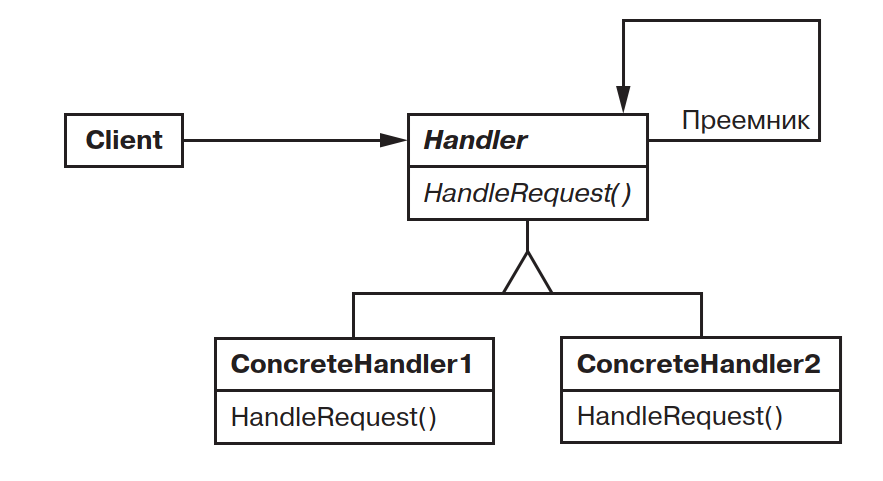
\includegraphics[width=0.8\textwidth]{eolang/tr-02/assets/Picture9.png}
  \caption{Chain of responsibility Design Pattern}
  \label{fig:9}
\end{figure*}

\subsubsection{Participants}
\begin{enumerate}
    \item Handler —  handler: defines the interface for processing requests; (optionally) implements communication with the successor.
    \item ConcreteHandler — specific handler: processes the request for which it is responsible; Has access to his successor; If ConcreteHandler  is able to process the request, it does so, if it cannot, it sends it to its successor;
    \item Client: Sends a request to some ConcreteHandler object in the chain.
\end{enumerate}

\subsubsection{Relation}
A request initiated by a client is moved along the chain until some ConcreteHandler object takes responsibility for processing it.

\subsubsection{Implementation}
\begin{verbatim}
1.	+package sandbox
2.	+alias stdout org.eolang.io.stdout
3.	+alias sprintf org.eolang.txt.sprintf
4.	
5.	[nextHandler] > defaultHandler
6.	  [message] > process
7.	    "" > @
8.	
9.	[] > handler1
10.	  [message] > process
11.	    if. > @
12.	      message.eq "1"
13.	      "one"
14.	      ^.nextHandler.process message
15.	  defaultHandler > @
16.	    handler2
17.	
18.	[] > handler2
19.	  [message] > process
20.	    if. > @
21.	      message.eq "2"
22.	      "two"
23.	      ^.nextHandler.process message
24.	  defaultHandler > @
25.	    handler3
26.	
27.	[] > handler3
28.	  [message] > process
29.	    if. > @
30.	      message.eq "3"
31.	      "three"
32.	      ^.nextHandler.process message
33.	  defaultHandler > @
34.	    handler4
35.	
36.	[] > handler4
37.	  [message] > process
38.	    if. > @
39.	      message.eq "4"
40.	      "four"
41.	      ^.nextHandler.process message
42.	  defaultHandler > @
43.	    defaultHandler
44.	
45.	[args...] > appChain
46.	  handler1 > hChain
47.	  stdout > @
48.	    sprintf
49.	      "%s\n"
50.	hChain. process
51.	        args.get 0 

\end{verbatim}


The input parameter args[0] is passed sequentially to 4 handlers, each of which processes its value (numbers from 1 to 4 are converted into words if another parameter is entered, an empty string is returned).

\subsection{Command}
Command pattern is a behavioral design pattern.

\subsubsection{Purpose}
Encapsulates a query in an object, thereby allowing clients to be parameterized  for different requests, queued or logged requests, and supports cancellation of operations.

\subsubsection{Structure}
See fig. \ref{fig:11}
\begin{figure*}[!t]
  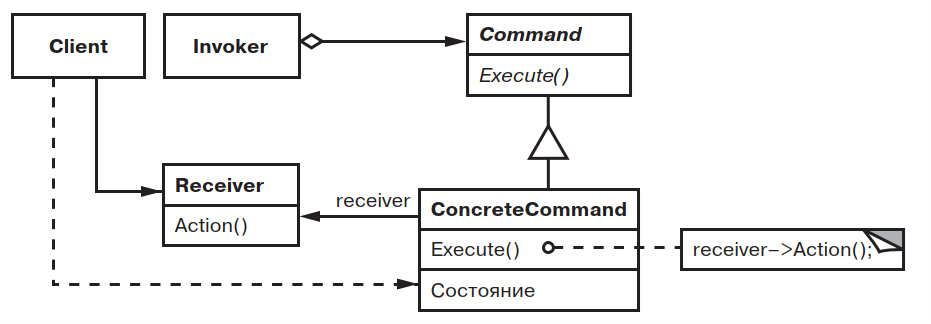
\includegraphics[width=0.8\textwidth]{eolang/tr-02/assets/Picture11.png}
  \caption{Command Design Pattern}
  \label{fig:11}
\end{figure*}

\subsubsection{Participants}
\begin{enumerate}
    \item - Command — command: declares the interface to perform the operation.
    \item -	ConcreteCommand is a specific  team: defines the relationship between the Receiver receiving object and the action; implements the Execute operation by calling the corresponding operations of the  Receiverobject.
    \item — Client— client: Creates a ConcreteCommand class object and sets its recipient.
    \item - Invoker— initiator: calls the command to execute the request.
    \item - Receiver  — recipient: has information about how to perform the operations necessary to meet the request. Any class can act as a recipient.
\end{enumerate}

\subsubsection{Relations}
\begin{enumerate}
    \item - The client creates a ConcreteCommand object and sets a recipient for it.
    \item - The Invoker initiator saves the  ConcreteCommandobject.
    \item - The initiator sends a request by calling the ExecuteCommandOperation. If undoing of actions performed is supported, ConcreteCommand  stores sufficient status information to perform the cancellation before calling  Execute.
    \item - The ConcreteCommand  object  invokes the recipient's operations to execute the request.
\end{enumerate}

\subsection{Null}
The Null Object Pattern is one of the behavioral design patterns.

\subsubsection{Purpose}
Null object pattern is used to replace check of NULL object instance to simplify the use of dependencies that can be undefined.

\subsubsection{Problem}
In Null Object pattern, a null object replaces check of NULL object instance. Instead of putting if check for a null value, Null Object reflects a do-nothing relationship. Such Null object can also be used to provide default behaviour in case data is not available. The concept of null objects comes from the idea that some methods return null instead of real objects and may lead to having many checks for null in your code. 


In Java and C++, the key to the Null Object pattern is an abstract class that defines the interface for all objects of this type. The Null Object is implemented as a subclass of this abstract class. Because it conforms to the abstract class' interface, it can be used any place this type of object is needed. Null object should not have any state.


In Eolang, the concept of null does not exist as every object is meant to dataize to a value, and as such given a value on creation. As classes and interfaces do not exist here either, the closest implementation in Eolang would be to have every object implement a null attribute that either dataizes to a Boolean or a string representing a lack of value/data or whatever the default value of an object may be. In this case, there may still be checks to see if null is true or false or contains the expected string.

\subsubsection{Implementation}
\begin{verbatim}
1.	+package sandbox
2.	+alias sprintf org.eolang.io.sprintf
3.	
4.	[] > null
5.	  "null" > @
6.	
7.	[args...] > appNull
8.	  sprintf > @
9.	    if.
10.	      args.isEmpty
11.	      null
12.	      args.get 0 

\end{verbatim}

\textbf{output:}


run.cmd
null

\subsection{Decorator}
Decorator is a structural design pattern.

\subsubsection{Purpose}
Decorator pattern allows you attach new behaviors to objects by placing these objects inside special wrapper objects that contain the behaviors.

\subsubsection{Problem}
Decorator pattern allows a user to add new functionality to an existing object without altering its structure. This pattern creates a decorator class which wraps the original class and provides additional functionality keeping class methods signature intact.


In Eolang, a copy of an object can be made, and new functionality be added. Here, the original object represents the decorator.

\subsubsection{Implementation}
\begin{verbatim}
1.	+package sandbox
2.	+alias sprintf org.eolang.io.sprintf
3.	
4.	[] > carsDecorate
5.	  8 > @
6.	
7.	[num] > someCars
8.	   decorateWithMoreCars num > @
9.	
10.	   [number] > decorateWithMoreCars
11.	     add. > @
12.	       carsDecorate
13.	       number
14.	
15.	[args...] > appDecorator
16.	  stdout > @
17.	    someCars (args.get 0) 

\end{verbatim}

In this example, the object “someCars” increases the number of cars in decarDecorator is for itself.

\textbf{Output}


run.cmd 5
13

It can be concluded that decorator design pattern naturally exits in Eolang.

\subsection{Builder}
Suppose, we have a class with a variety of input parameters. The input parameters are used to configure instances of the class. Some of the parameters may be optional, while some of them are mandatory to be sat up. Hence, the following techniques of configuration of instances of the class may be applied:
\begin{enumerate}
    \item Configuration of instance variables of an object directly in the user code through Setter Methods calls or by referencing variables straightforwardly. This practice may not be considered appropriate because it makes code instances more cohesive and interdependent while violating encapsulation of the inner state of objects (which may lead to breaking of the integrity of business logic of an application), and, hence, the usage of the practice is not encouraged. In addition, this technique may allow situations in which objects are being in an incomplete state, which also may break the logic of an application.
    \item Creation of subclasses of the considered class when each successor has a slightly changed prototype of its constructors. This technique implies that prototypes of constructors of different subclasses have subsets of optional parameters in them while omitting some parameters, which makes it possible to create configurable instances of objects in a controlled manner. This practice is more encouraged to be applied in practice since it implies control over the creational process. However, it is not recommended for use when choosing the sole parent superclass is challenging or when the practice produces a wide or deep hierarchy of inheritance
    \item Overloading of constructors or setting a single constructor with optional parameters. While this practice allows classes to create instances in a controlled way, it is undesirable in cases where the number of parameters or constructor overloads is too large to be manageable and understandable.
\end{enumerate}

The Builder pattern may be considered a universal solution to the problem. The pattern defines the Builder class, which has methods (stages) for building objects. The user code can call the stages in any order, omitting some of them (optional configurations). Also, the Builder class may check that all the required parameters are set up. At the end of construction, user code is required to call a method that finishes the construction process and returns a ready-made object. The pattern encapsulates the creational sensitive logic inside the Builder class and makes the configuration process manageable to the user code.

\subsubsection{Structure}
See fig. \ref{fig:01}.
\begin{figure*}[!t]
  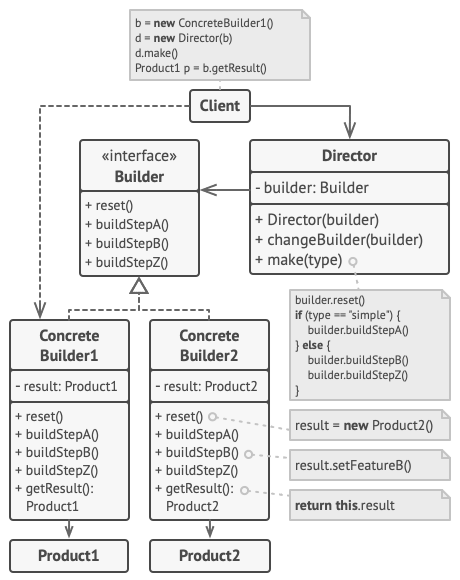
\includegraphics[width=0.8\textwidth]{eolang/tr-02/assets/Picture01.png}
  \caption{Builder Design Pattern}
  \label{fig:01}
\end{figure*}

\subsubsection{Code Instances Involved}
Builder is an abstract class that defines the contract of the creational steps of Products for its successors (concrete builders). Also, the Builder superclass defines the finizaliotion method. 
Product is an interface for products (instances being created and configured through the Builder pattern). The interface defines the contract for all products so that these may be managed by Builders.
(optional) Director is a class, which defines higher-level (that is, higher than the level of "understanding" of the builder itself, for example, rules for mandatory fields and compliance with business logic) scripts for building objects. The director can be used to reuse some high-level business logic for constructing objects based on various builder implementations.

\subsubsection{Relations}
Implementations of the Product interface are products. Inheritors of the Builder class provide concrete implementations for the building steps (or borrow some of those steps from the superclass). The Director (optional entity) class can manage builders in a general style (based on some configuration) in accordance with the higher-level logic of business rules. The client code can contact the Director, giving it the configuration, or build an object using the Builder directly.

\subsubsection{Implementation}
First, we should mention that the problem solved by the Builder pattern may be addressed by the partial application mechanism embedded into the language as one of its features. The partial application mechanism allows programmers to partially apply objects (i.e., create objects with some or all of the input attributes omitted and then, optionally, set unbound attributes after throughout the program). This technique may be utilized as a more concise alternative to constructor overloading. Here is an example:
\begin{verbatim}
[a b c name] > triangle
  add. > perimeter
    add.
      a
      b
    c

  sprintf > toString
    "The triangle is named '%s'."
    name


[args...] > app
  triangle > triangleA
    10:a
  triangleA > triangleABC
    7:b
    8:c
  triangleABC > triangleABCNamed
   "My Triangle":name
  triangle > triangleNamed
    "My Another Triangle":name

\end{verbatim}


Here, we have the triangle object with input attributes a, b, c, and name. The triangle object has two bound attributes: perimeter (which relies on a, b, and c) and toString (which relies on name). Object app demonstrates the partial application mechanism. So, triangleA has only the a attribute bound, triangleABC has all the sides (a, b, c) sat up, triangleABCNamed has all the sides and its name configured, and triangleNamed has the name only. All three triangles are constructed through partial application (meaning, some of the attributes are left unbound or were bound after). The above example demonstrates an alternative solution to the problem of optional configuration of objects. However, this solution does not encapsulate the creation process of objects. Hence, the Builder pattern still may have its place in the EO environment.

Consider the following example:

\begin{verbatim}
[] > builder
  subbuilder triangle > @
  [triangleEntity] > subbuilder
    # finalizes the construction process
    [] > finalize
      ^.^.subbuilder > @
    # configures the a free attribute
    [aVal] > setA
      ^.^.subbuilder > @
        ^.^.triangleEntity
          (^.validateSide aVal):a
    # configures the b free attribute
    [bVal] > setb
      ^.^.subbuilder > @
        ^.^.triangleEntity
          (^.validateSide bVal):b
    # configures the c free attribute
    [cVal] > setc
      ^.^.subbuilder > @
        ^.^.triangleEntity
          (^.validateSide cVal):c
    # configures the name free attribute
    [nameVal] > setname
      ^.^.subbuilder > @
        ^.^.triangleEntity
          (^.validateName nameVal):name
    # validates side value
    [val] > validateSide
      if. > @
        val.greater 0
        val
        error
          "The side of a triangle must not be less than 1!"
    # validates name
    [val] > validateName
      if. > @
        val.length.neq 0
        val
        error
          "The name of a triangle must not be empty!"

[args...] > app
  builder > b
  finalize. > triangleABC
    setC.
      setB.
        setA.
          builder
          10
        12
      0

\end{verbatim}


Here we implemented the principles of the Builder pattern through measures supplied by the EO language. The builder object contains the subbuilder attribute object that implements the construction steps (setA, setB, setC, setName) as well as validation sub-steps (validateSide, validateName) and the finalize attribute that finishes the construction process and returns the resulting object. Initially, the instantiation of the builder object is substituted with a copy of the subbuilder object with an empty (meaning, all free attributes are unbound) copy of the constructing object. On each construction step, the subbuilder object returns itself by passing a changed version of the constructing object to its constructor. The construction steps have validation substeps that may implement some complex business logic. Validation steps may return an error or a validated object, which may lead to an interruption of the program execution and prevent inconsistency of the business logic.
In conclusion, we would like to notice that the problem originally stated above (problem of optional configuration of objects with a lot of input parameters) and solved with the Builder pattern may not be actual to EO since it has the partial application mechanism that allows programmers to perform such configuration and, in addition, EO does not allow objects to have more than four free attributes (although, this restriction may be mitigated through passing complex object structures as free attributes). Nevertheless, the EO implementation of the Builder pattern may find its utilization in scopes where encapsulation of the creational process of objects is required. For instance, it may be needed when business logic validation of values passed for binding to free attributes is required.


\subsection{Factory Method}
The Factory Method Pattern is a creational object-oriented design pattern.

\subsubsection{Purpose}
Defines the creational method in the Creator superclass that defines a rule (that is, an interface or a contract) for creating an object (product) of some supertype Product. This method is used by the superclass or its more specific implementations, and the factory method can also be called from outside the class by other entities within the application. Concrete implementations of the Creator class with a factory method can return subtypes of the Product type, thereby "tailoring" a specific implementation of the product class to the one required by the factory method contract. Hence, the pattern allows programmers to implement seamless configuration of the architecture of the application.

\subsubsection{Problem}
The pattern addresses the problem of extending the architecture of an application. By specifying  the product contract (Product Interface) and by defining the class contract with the Factory Method Class, the architect separates the responsibility for creating the product itself from other methods of the creator class. This can be useful when:
\begin{enumerate}
    \item It is not known what types of the Product class may be used in the future, but it may be appropriate to leave a headroom for a potential extension of the application architecture. Otherwise, this can be interpreted as an implementation of the "Open / Closed” principle (O in SOLID).
    \item Implementation of the principle of "Single Responsibility" (S in SOLID). The code responsible for setting (configuring) a specific version of the product can be placed in a single place, for example, in a class that configures the application based on the environment settings. Here, the Dependency Injection mechanism can also be used to perform such a configuration in an invisible manner.
    \item The pattern allows programmers to separate the logic of product creation from other logic of the creator class. This facilitates the reuse of identical code.
\end{enumerate}

\subsubsection{Structure}
See fig. \ref{fig:02}.
\begin{figure*}[!t]
  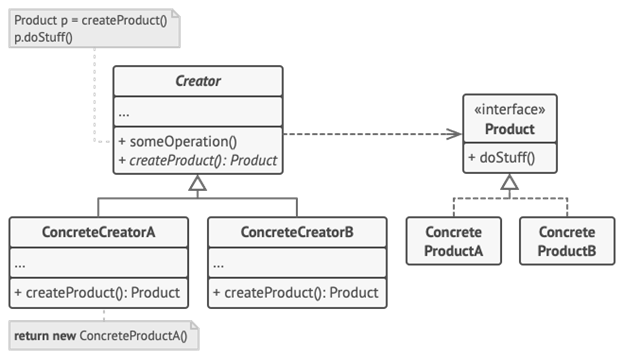
\includegraphics[width=0.8\textwidth]{eolang/tr-02/assets/Picture02.png}
  \caption{Factory Method Design Pattern}
  \label{fig:02}
\end{figure*}

\subsubsection{Code Instances Involved}
Creator is an abstract class that defines the contract of the reutilized steps (here, it is someOperation) and the creational step (createProduct) of Products for its successors (concrete creators). 
Product is an interface for products (instances being created and configured through the Factory Method pattern). The interface defines the contract for all products so that these may be managed by the pattern.

\subsubsection{Relation}
Implementations of the Product interface are products. Inheritors of the Creator class provide concrete implementations for the creational method and inherit the rest methods. The concrete implementation of the creational method may return different implementations of Product, which implies the substitution of logic (or configurability of the application). 

\subsubsection{Implementation}
The EO programming language does not have interfaces, classes, and types. Because of it, we may omit defining the Product interface contract (since it would not impose any requirements). Consider the following implementation of the pattern in EO: 

\begin{verbatim}
[] > creator
  # left to be redefined
  [] > createObject
  # operation over products
  [] > performOperation
    createObject.getWeight.add 1 > @

[] > concreteCreatorA
  creator > @
  [] > createObject
    productA > @

[] > concreteCreatorB
  creator > @
  [] > createObject
    productB > @

[] > productA
  # let's suppose that this implementation
  # gets value from the production server
  [] > getWeight
    42 > @

[] > productB
  # let's suppose that this implementation
  # gets value from the testing server
  [] > getWeight
          24 > @

\end{verbatim}

Here, we have the creator object with the performOperation attribute (the logic to be reused) and the createObject attribute (the logic to be redefined for flexible substitution of objects). The concreteCreatorA and concreteCreatorB objects have the creator object as their decoratee, so that these might inherit the reusable logic. Both objects define the createObject attribute that hides the original attribute of the same name from the decoration hierarchy. Objects productA and productB implement the attribute of interest (getWeight) differently. One of them may get the value from the production server, while another takes it from the testing environment. This example demonstrates the implementation of the classic version of the pattern in EO. However, we may consider a more EO-idiomatic example, free from additional structures (concrete creators) utilized in statically typed class-based object-oriented languages such as Java or C++. Consider the following example: 

\begin{verbatim}
[@] > creator
  # operation over products
  [] > performOperation
    createObject.getWeight.add 1 > @

[] > productA
  # let's suppose that this implementation
  # gets value from the production server
  [] > getWeight
    42 > @

[] > productB
  # let's suppose that this implementation
  # gets value from the testing server
  [] > getWeight
    24 > @

[args...] > app
  creator > creatorObject
    []
      [] > createObject
        if. > @
          (args.get 0).eq "test"
          productB
          productA

\end{verbatim}

Here, we used the technique of passing decoratee as a free attribute of the object creator. Its decoratee is passed in the app object. The decoratee has the only attribute createObject that the creator object inherits and relies on. The createObject attribute decides what version of a product should be chosen based on the environment configuration. This implementation of the pattern may be considered as more idiomatic and flexible from the EO perspective.


\subsection{The Closures Functional Programming Technique}
Since the EO programming language may be considered semi-functional, it might be useful to apply one of the widely adopted functional programming techniques, closures, in it. Simply put, the closures mechanism implies capturing outer lexical scope variables inside a function defined inside the scope with a consequent utilization of the function in other scopes. To support this technique, a language must operate over function as if they are first-class citizens (i.e., a language must return function or pass functions as parameters). Here is an example of this technique in JavaScript:

\begin{verbatim}
function makeAdder(x) {
  return function(y) {
    return x + y;
  };
}
var add5 = makeAdder(5);
var add10 = makeAdder(10);
console.log(add5(2));  // 7
console.log(add10(2)); // 12
\end{verbatim}

Here, we have the makeAdder function that returns an anonymous function capturing its outer state x. The state is then utilized when the returned function is applied with its own parameter y. In other words, the inner anonymous function remembers the value of x and uses it even when the actual value disappeared from the stack. This technique may be useful to emulate access modificators in functional languages: 

\begin{verbatim}
var counter = (function() {
  var privateCounter = 0;
  function changeBy(val) {
    privateCounter += val;
  }

  return {
    increment: function() {
      changeBy(1);
    },

    decrement: function() {
      changeBy(-1);
    },

    value: function() {
      return privateCounter;
    }
  };
})();

console.log(counter.value());  // 0.

counter.increment();
counter.increment();
console.log(counter.value());  // 2.

counter.decrement();
console.log(counter.value());  // 1.
\end{verbatim}

Here, the outer function counter returns a complex object-like structure containing functions that capture the state of the counter function. The state of the counter function is also complex: it has a mutable local variable privateCounter, and the changeBy function that mutates the value in the unified manner. The user code may not access the value and the mutating functions directly: both of them disappeared from the stack. However, the closures returned by the outer function still may do it. Hence, the technique allows functional programmers to simulate private state. 

We surely may reproduce the similar technique of capturing the lexical scope in EO:
\begin{verbatim}
[] > counter
  memory 0 > privateCounter
  [val] > changeBy
    privateCounter.write > @
      privateCounter.add val
  [] > @
    [] > increment
      ^.^.changeBy 1 > @
    [] > decrement
      ^.^.changeBy (-1) > @
    [] > value
      ^.^.privateCounter > @

\end{verbatim}



\section{Conclusion}
It is possible to conclude that (1) EO is principally applicable to all the considered patterns; (2) For some patterns, EO is able to give a fairly concise and intuitively clear code, since the language combines the features of Functional Programming and OOP; (3) the issues of effective implementation of patterns on EO are largely determined by the characteristics of the environment (IDE + compiler) and today remain open.

Also, EO has no local variables or any kind of stack-lifetime storage. Instead, any name refers to an object (stored in heap) that may be accessed through the scope of any other object via the dot-notation mechanism. Even anonymous objects may allow programmers to access its local scope (including parent and decoration hierarchies) freely. In addition, EO has no access modification instruments. This makes closures technique almost similar to the partial application mechanism. Moreover, the publicity of any attribute of any object makes encapsulation impossible in the language. This differentiates EO from functional programming languages and, also, from object-oriented languages. Absence of instruments of access modification (or simulation of it) may be a severe violation of object-oriented principle of encapsulation, which may lead to insecure environments breaking business logic of problem domains.

EO is fundamentally applicable to all the patterns considered. 2) For some patterns, EO is able to give a fairly concise and intuitively clear code, since the language combines the features of Functional Program (FP) and OOP. 3) the issues of effective implementation of patterns on EO are largely determined by the characteristics of the environment (IDE + compiler).

The implementation of the design patterns in Eolang is available at \cite{1093892.2389691/8768226502}.


\bibliographystyle{ACM-Reference-Format}
\raggedright
\bibliography{main}
\clearpage


\end{document}
